\Variant{03.10.2026 (1-smena)}
\QQ{1}{$\overline{34b5a}$ beş xonali son $36$ ga qoldiqsiz bölinadi. Bunday $(a;\,b)$ juftliklar neçta?
\Opts{$2$ ta}{$1$ ta}{$3$ ta}{$4$ ta}}
\QQ{2}{$2^7+4^4+16^3$ ifodaning qiymati quyidagilardan qaysi biriga qoldiqsiz bölinadi?
\Opts{$13$}{$7$}{$17$}{$11$}}
\QQ{3}{Töqqizinçi sinf öquvçilari $100$ nafar. Öquvçilardan $84$ tasi matematika tögaragiga, $68$ tasi ingliz tili tögaragiga, $72$ tasi fizika tögaragiga qatnaşadi. Uççala tögarakka ham qatnaşadigan öquvçilar eng kamida neçta böladi?
\Opts{$20$}{$24$}{$16$}{$32$}}
\QQ{4}{Ikkita guruh birgalikda işlab, ajratilgan yölni $6$ kunda taʼmirlab tugatadi. Birinçi guruh yolğiz işlab yölning $40\%$ ini taʼmirlaşi uçun ikkinçi guruh yolğiz işlab yölning $13\frac13\%$ ini taʼmirlaşiga qaraganda $2$ kun köp vaqt sarflaydi. Birinçi guruh yolğiz işlasa, yölni neça kunda taʼmirlaydi?
\Opts{$12$}{$15$}{$10$}{$8$}}
\QQ{5}{Hisoblang:
\[\frac{2^5\cdot3^8\cdot7^5+243\cdot14^5\cdot48}{625\cdot98\cdot6^5-2^5\cdot3^5\cdot35^2}\]
\Opts{$\dfrac{220}9$}{$15$}{$21$}{$\dfrac{220}{13}$}}
\QQ{6}{Hisoblang:
\[\sqrt{31\cdot30\cdot29\cdot28+1}\]
\Opts{$871$}{$868$}{$869$}{$870$}}
\QQ{7}{Hisoblang:
\[\left(3\sqrt3+\sqrt{15}+6+2\sqrt5\right)\left(3\sqrt3-\sqrt{15}-6+2\sqrt5\right)\]
\Opts{$4$}{$-2$}{$2$}{$-4$}}
\QQ{8}{Arifmetik progressiyada $a_{11}=24$ bölsa, $S_{21}$ ni toping.
\Opts{$504$}{$480$}{$528$}{$252$}}
\QQ{9}{Ösuvçi geometrik progressiyaning birinçi, ikkinçi va uçinçi hadlari mos ravişda $x+3$, $x+7$ va $2x+8$ ga teng. Geometrik progressiyaning beşinçi hadini toping.
\Opts{$27$}{$36$}{$60{,}75$}{$40{,}5$}}
\QQ{10}{Ifodani soddalaştiring:
\[\frac a{a^2+b^2}-\frac{b(a-b)^2}{a^4-b^4}\]
\Opts{$\dfrac1{a-b}$}{$\dfrac1{a+b}$}{$\dfrac a{a+b}$}{$\dfrac{a-b}{a^2+b^2}$}}
\QQ{11}{Agar $x>12$ bölsa, ifodani soddalaştiring:
\[\sqrt{x+6+6\sqrt{x-3}}-\sqrt{x+6-6\sqrt{x-3}}\]
\Opts{$2\sqrt{x-3}$}{$-6$}{$6$}{$2x$}}
\QQ{12}{$a$ ning neçta butun qiymatida $4\sin2x-6\cos2x=a$ tenglama yeçimga ega?
\Opts{$14$ ta}{$15$ ta}{$13$ ta}{$7$ ta}}
\QQ{13}{Tenglamaning $\left[\dfrac\pi2;\,\dfrac{5\pi}2\right]$ oraliğidagi ildizlari yiğindisini toping:
\[\frac{\sin x+1}{\sin x-1}=\cos x\]
\Opts{$\dfrac{3\pi}2$}{$4\pi$}{$\dfrac{5\pi}2$}{$\dfrac{7\pi}2$}}
\QQ{14}{Tenglama neçta haqiqiy ildizga ega?
\[3\cdot9^x+4\cdot25^x=7\cdot15^x\]
\Opts{$1$ ta}{haqiqiy ildizga ega emas}{$3$ ta}{$2$ ta}}
\QQ{15}{$x^2-3|x|+2=0$ tenglama neçta haqiqiy ildizga ega?
\Opts{$4$ ta}{$2$ ta}{$3$ ta}{$1$ ta}}
\QQ{16}{Tengsizlikni qanoatlantiruvçi butun sonlar yiğindisini toping:
\[|x-1|+|2-x|\le1\]
\Opts{$1$}{$3$}{$2$}{$6$}}
\QQ{17}{Tenglama neçta haqiqiy ildizga ega?
\[2025^x+2026\cdot2025^{1-x}=4051\]
\Opts{$2$ ta}{$1$ ta}{$3$ ta}{haqiqiy ildizga ega emas}}
\QQ{18}{Tengsizlikni qanoatlantiruvçi butun sonlar yiğindisini toping:
\[\log_3\left(2^x-1\right)+\log_{2^x-1}3\le3\frac13\]
\Opts{$9$}{$10$}{$7$}{$5$}}
\QQ{19}{Tengsizlikni yeçing:
\[\Bigl||x^2-6x+8|-3\Bigr|\ge x-1\]
\Opts{$(-\infty;\,3]\cup(6;\,+\infty)$}{$(-\infty;\,3]\cup\{4\}\cup[6;\,+\infty)$}{$(-\infty;\,2]\cup[6;\,+\infty)$}{$(-\infty;\,4]\cup(6;\,+\infty)$}}
\QQ{20}{$f(x)$ — davriy funksiya, uning eng kiçik musbat davri $3$ ga teng va $f(2)=5$. $f(8)+f(-4)-f(-1)$ ni hisoblang.
\Opts{$10$}{$0$}{$5$}{$15$}}
\QQ{21}{Rasmda $y=ax^3+bx^2+cx+d$ funksiyaning grafigi berilgan. Funksiya grafigi koordinatalar boşidan ötadi va $Ox$ öqiga $(2;\,0)$ nuqtada urinadi. $f(-2)$ ni toping.
\qfig{\begin{tikzpicture}[xscale=1.2,yscale=1.1,font=\small]
\draw[-{Stealth[length=4pt]}] (-0.6,0)--(3.4,0) node[right] {$x$}; \draw[-{Stealth[length=4pt]}] (0,-1.6)--(0,2.2) node[left] {$y$};
\draw[thick,domain=-0.3:2.75,samples=80] plot (\x,{\x*(\x-2)*(\x-2)});
\fill (0,0) circle (1.5pt); \fill (2,0) circle (1.5pt); \fill (0.667,1.185) circle (1.5pt);
\node[above] at (0.667,1.2) {$\left(\frac23;\,\frac{32}{27}\right)$}; \node[below left] at (0,0) {$(0;\,0)$}; \node[below] at (2,0) {$(2;\,0)$};
\end{tikzpicture}}
\Opts{$-32$}{$-16$}{$-8$}{$-24$}}
\QQ{22}{$f(x)=\dfrac{x+3}{(x-4)\sqrt{x-4}}$ funksiyaning boşlanğiç funksiyasi $F(x)$ bölsin. $F(x)$ funksiya grafigi $(5;\,0)$ nuqtadan ötsa, $F(8)$ ni toping.
\Opts{$5$}{$-3$}{$12$}{$9$}}
\QQ{23}{$ABC$ uçburçakda $\angle A=76^\circ$ va $\angle B=67^\circ$. $A$ uçidan $BC$ tomonga $AD$ balandlik tuşirilgan. $AB$ tomonda yotuvçi ixtiyoriy $F$ nuqtadan $AC$ tomonga $FE$ perpendikulyar ötkazilgan. $AD$ va $FE$ töğri çiziqlar kesişişidan hosil bölgan ötkir $\alpha$ burçakni toping.
\qfig{\begin{tikzpicture}[scale=0.62,font=\small]
\coordinate (A) at (0,0); \coordinate (C) at (8,0); \coordinate (B) at (1.265,5.075); \coordinate (D) at (2.897,3.845); \coordinate (F) at (0.759,3.045); \coordinate (E) at (0.759,0); \coordinate (P) at (0.759,1.007);
\draw (A)--(B)--(C)--cycle; \draw (A)--(D); \draw (F)--(E);
\draw ($(D)!0.3cm!(A)$)--($(D)!0.3cm!(A)+(D)!0.3cm!(C)-(D)$)--($(D)!0.3cm!(C)$); \draw (0.759,0.3)--(1.059,0.3)--(1.059,0);
\draw ($(P)+(90:0.45)$) arc[start angle=90,end angle=53,radius=0.45]; \node at ($(P)+(72:0.75)$) {\scriptsize$\alpha$};
\node[below left] at (A) {$A$}; \node[above] at (B) {$B$}; \node[below right] at (C) {$C$}; \node[above right] at (D) {$D$}; \node[left] at (F) {$F$}; \node[below] at (E) {$E$}; \node[left] at (P) {$P$};
\end{tikzpicture}}
\Opts{$37^\circ$}{$53^\circ$}{$143^\circ$}{$23^\circ$}}
\QQ{24}{$f(x)$ funksiya uçun $f\left(\dfrac{3+x}{1-x}\right)+f\left(\dfrac{x-3}{x+1}\right)=x$ bölsa, $f'(0)$ ni toping.
\Opts{$4$}{$\dfrac72$}{$-4$}{$\dfrac12$}}
\QQ{25}{$OAC$ töğri burçakli uçburçakda $\angle OAC=90^\circ$, $\angle AOC=30^\circ$ va $OA=10$. Markazi $O$ nuqtada, radiusi $OA$ ga teng bölgan aylana yoyi $OC$ gipotenuzani $B$ nuqtada kesadi. Böyalgan soha yuzini toping.
\qfig{\begin{tikzpicture}[scale=0.42,font=\small]
\fill[qfill] (8.66,5)--(10,5.774)--(10,0) arc (0:30:10)--cycle;
\draw (0,0)--(10,0)--(10,5.774)--cycle; \draw (10,0) arc (0:30:10);
\draw (1.5,0) arc (0:30:1.5); \node at (2.4,0.6) {\scriptsize$30^\circ$};
\node[left] at (0,0) {$O$}; \node[below right] at (10,0) {$A$}; \node[above right] at (10,5.774) {$C$}; \node[above left] at (8.66,5) {$B$}; \node[below] at (5,0) {$10$};
\end{tikzpicture}}
\Opts{$\dfrac{50\sqrt3+25\pi}3$}{$\dfrac{100\sqrt3-50\pi}3$}{$\dfrac{50\sqrt3-25\pi}3$}{$\dfrac{25\sqrt3+25\pi}3$}}
\QQ{26}{$ABC$ uçburçakning $AB$ va $AC$ tomonlari mos ravişda $9$ va $6$ ga teng. $A$ uçidan $BC$ tomonga $AM$ mediana va $AI$ bissektrisa ötkazilgan. Agar $BM=5$ bölsa, $AMI$ uçburçak yuzini toping.
\qfig{\begin{tikzpicture}[scale=0.45,font=\small]
\coordinate (B) at (0,0); \coordinate (C) at (10,0); \coordinate (A) at (7.25,5.333); \coordinate (M) at (5,0); \coordinate (I) at (6,0);
\fill[qfill] (A)--(M)--(I)--cycle; \draw (A)--(B)--(C)--cycle; \draw (A)--(M); \draw (A)--(I);
\node[above] at (A) {$A$}; \node[below left] at (B) {$B$}; \node[below right] at (C) {$C$}; \node[below] at (M) {$M$}; \node[below] at (I) {$I$};
\node[above left] at (3.6,2.7) {$9$}; \node[above right] at (8.6,2.7) {$6$}; \node[below] at (2.5,0) {$5$};
\end{tikzpicture}}
\Opts{$\dfrac{\sqrt{455}}8$}{$\dfrac{\sqrt{455}}4$}{$\dfrac{3\sqrt{455}}4$}{$\dfrac{\sqrt{455}}2$}}
\QQ{27}{$ABCD$ ($BC\parallel AD$) teng yonli trapetsiyaning diagonallari $O$ nuqtada töğri burçak ostida kesişadi. $P$, $E$ va $F$ nuqtalar mos ravişda $AB$, $AC$ va $BD$ kesmalarning örtalari. Agar $CD=4\sqrt5$ va $EF=4$ bölsa, $APO$ uçburçak yuzini toping.
\qfig{\begin{tikzpicture}[scale=0.4,font=\small]
\coordinate (A) at (0,0); \coordinate (D) at (12,0); \coordinate (B) at (4,8); \coordinate (C) at (8,8); \coordinate (O) at (6,6); \coordinate (P) at (2,4); \coordinate (E) at (4,4); \coordinate (F) at (8,4);
\fill[qfill] (A)--(P)--(O)--cycle;
\draw (A)--(B)--(C)--(D)--cycle; \draw (A)--(C); \draw (B)--(D); \draw (E)--(F); \draw (P)--(O);
\draw ($(O)!0.5cm!(C)$)--($(O)!0.5cm!(C)+(O)!0.5cm!(D)-(O)$)--($(O)!0.5cm!(D)$);
\node[below left] at (A) {$A$}; \node[above left] at (B) {$B$}; \node[above right] at (C) {$C$}; \node[below right] at (D) {$D$}; \node[above] at (O) {$O$};
\node[left] at (P) {$P$}; \node[below] at (E) {$E$}; \node[below] at (F) {$F$}; \node[above] at (6,4) {$4$}; \node[right] at (10,4) {$4\sqrt5$};
\end{tikzpicture}}
\Opts{$12$}{$8$}{$4$}{$6$}}
\QQ{28}{$ABCDE$ muntazam beşburçakning $AC$ diagonali $ACTR$ rombning tomoniga teng, $R$ nuqta $AE$ nurida yotadi. Çizmadagi maʼlumotlarga asoslanib, $x$ burçakni toping.
\qfig{\begin{tikzpicture}[scale=0.95,font=\small]
\coordinate (A) at (0,0); \coordinate (E) at (2,0); \coordinate (D) at (2.618,1.902); \coordinate (C) at (1,3.078); \coordinate (B) at (-0.618,1.902); \coordinate (R) at (3.236,0); \coordinate (T) at (4.236,3.078);
\draw (A)--(B)--(C)--(D)--(E)--cycle; \draw (A)--(C)--(T)--(R)--cycle; \draw (C)--(R);
\draw ($(C)+(-54:0.9)$) arc[start angle=-54,end angle=-36,radius=0.9]; \node at ($(C)+(-45:1.2)$) {\scriptsize$x$};
\node[below left] at (A) {$A$}; \node[left] at (B) {$B$}; \node[above] at (C) {$C$}; \node[right] at (D) {$D$}; \node[below] at (E) {$E$}; \node[below] at (R) {$R$}; \node[above right] at (T) {$T$};
\end{tikzpicture}}
\Opts{$18^\circ$}{$15^\circ$}{$30^\circ$}{$9^\circ$}}
\QQ{29}{Tekislikni kesib ötmaydigan $AB$ kesmaning uçlaridan tekislikkaça bölgan masofalar $AA_1=9$ sm va $BB_1=19$ sm. $AB$ kesmada $C$ nuqta olingan bölib, u kesmani $AC:CB=3:4$ nisbatda böladi. $C$ nuqtadan tekislikkaça bölgan masofani toping.
\Opts{$\dfrac{93}7$ sm}{$13$ sm}{$\dfrac{97}7$ sm}{$14$ sm}}
\QQ{30}{$\vec a$ va $\vec b$ vektorlar uçun $|\vec a|=2$, $|\vec b|=4$ va ular orasidagi burçak $60^\circ$ ga teng. $2\vec a-3\vec b$ va $2\vec a-5\vec b$ vektorlarning skalyar köpaytmasini toping.
\Opts{$256$}{$192$}{$128$}{$160$}}
\QQ{31}{$A=\left\{x\in\mathbb Z\mid x^2>2025\right\}$ va $B=\left\{x\in\mathbb Z\mid |x|\le50\right\}$ töplamlar berilgan. $A\cap B$ töplamning qism töplamlari sonini toping.
\Opts{$32$}{$512$}{$1024$}{$2048$}}
\QQ{32}{$(x+2y)^5$ köphad standart şaklga keltirib yoyildi. Hosil bölgan köphad barça koeffitsiyentlarining yiğindisini toping.
\Opts{$32$}{$81$}{$729$}{$243$}}
\QQ{33}{\Moslash{Radiusi $R_1$ ga teng şarga öq kesimi kvadrat bölgan silindr içki çizilgan. Radiusi $R_2$ ga teng şarga öq kesimi muntazam uçburçak bölgan konus içki çizilgan. Silindr va konusning töla sirtlari teng.
\par\centering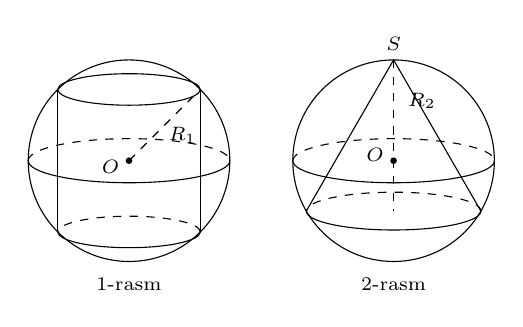
\begin{tikzpicture}[scale=0.8,font=\small]
\draw (0,0) circle (1.6); \draw[dashed] (-1.6,0) arc (180:0:1.6 and 0.35); \draw (-1.6,0) arc (180:360:1.6 and 0.35);
\draw (0,1.131) ellipse (1.131 and 0.25); \draw (-1.131,-1.131) arc (180:360:1.131 and 0.25); \draw[dashed] (1.131,-1.131) arc (0:180:1.131 and 0.25);
\draw (-1.131,-1.131)--(-1.131,1.131); \draw (1.131,-1.131)--(1.131,1.131); \draw[dashed] (0,0)--(1.131,1.131); \fill (0,0) circle (1.5pt);
\node[left] at (0,-0.1) {\scriptsize$O$}; \node at (0.85,0.4) {\scriptsize$R_1$}; \node[below] at (0,-1.7) {\scriptsize1-rasm};
\begin{scope}[xshift=4.2cm]
\draw (0,0) circle (1.6); \draw[dashed] (-1.6,0) arc (180:0:1.6 and 0.35); \draw (-1.6,0) arc (180:360:1.6 and 0.35);
\draw (-1.386,-0.8) arc (180:360:1.386 and 0.3); \draw[dashed] (1.386,-0.8) arc (0:180:1.386 and 0.3);
\draw (-1.386,-0.8)--(0,1.6)--(1.386,-0.8); \draw[dashed] (0,1.6)--(0,-0.8); \fill (0,0) circle (1.5pt);
\node[above] at (0,1.6) {\scriptsize$S$}; \node[left] at (0,0.1) {\scriptsize$O$}; \node at (0.45,0.95) {\scriptsize$R_2$}; \node[below] at (0,-1.7) {\scriptsize2-rasm};
\end{scope}
\end{tikzpicture}}{A) $\dfrac{\sqrt3}2$\par B) $\dfrac{\sqrt2}2$\par C) $\dfrac{\sqrt6}2$\par D) $\dfrac{\sqrt3}3$\par E) $\dfrac{\sqrt6}3$\par F) $\dfrac23$}{Silindr radiusining konus radiusiga nisbatini toping $\left(\dfrac{R_{\text{silindr}}}{R_{\text{konus}}}\right)$.}{Silindr hajmining konus hajmiga nisbatini toping $\left(\dfrac{V_{\text{silindr}}}{V_{\text{konus}}}\right)$.}{Birinçi şar radiusining ikkinçi şar radiusiga nisbatini toping $\left(\dfrac{R_1}{R_2}\right)$.}}
\QQ{36}{$a$ parametrning qanday qiymatida
\[\begin{cases}\log_3\left(x^4y^2+3a^2\right)=1+\log_3\left(1-ax^2y^2\right),\\ 2^{\frac y2}=4^{|x|+1}\end{cases}\]
sistema yagona yeçimga ega böladi?
\AB{$a$ ning barça haqiqiy qiymatlari yiğindisini toping (agar $a$ yagona bölsa, öşa qiymatni toping).}{Şu holda sistema yeçimi uçun $x+y$ ni toping.}}
\QQ{37}{Tenglamani yeçing:
\[\sin x+\sqrt3\cos x=1\]
\AB{Tenglamaning $[-2\pi;\,2\pi]$ oraliğidagi ildizlari yiğindisini toping.}{Tenglamaning $[0;\,5\pi]$ oraliğidagi ildizlari sonini toping.}}
\QQ{38}{$y=ax^2+bx+c$ parabolaga ikkita $y_1=k_1x+b_1$ va $y_2=k_2x+b_2$ urinmalar ötkazilgan. Uşbu urinmalarning parabolaga uriniş nuqtalari absissalari mos ravişda $x=3$ va $x=9$ ga teng. Urinmalar $Ox$ öqidagi $x=6$ nuqtada özaro kesişadi. Kesişiş nuqtasida urinmalar va $Ox$ öqi yoyiq burçakni uçta teng $\beta$ burçakka ajratadi.
\qfig{\begin{tikzpicture}[scale=0.5,font=\small]
\draw[-{Stealth[length=4pt]}] (-1,0)--(12,0) node[right] {$x$}; \draw[-{Stealth[length=4pt]}] (0,-2)--(0,10.5) node[left] {$y$};
\draw[thick,domain=1.2:10.8,samples=80] plot (\x,{0.2887*(\x-6)*(\x-6)+2.598}) node[above] {$y=ax^2+bx+c$};
\draw[domain=1.4:7.2,samples=2] plot (\x,{-1.732*(\x-6)}); \draw[domain=4.8:10.6,samples=2] plot (\x,{1.732*(\x-6)});
\fill (3,5.196) circle (2.5pt); \fill (9,5.196) circle (2.5pt);
\draw (7.2,0) arc (0:180:1.2); \node at (4.2,0.6) {\scriptsize$\beta$}; \node at (6,1.6) {\scriptsize$\beta$}; \node at (7.8,0.6) {\scriptsize$\beta$};
\draw (3,-0.15)--(3,0.15); \draw (9,-0.15)--(9,0.15); \node[below] at (3,0) {$3$}; \node[below] at (6,0) {$6$}; \node[below] at (9,0) {$9$};
\node[left] at (1.6,7.8) {$y_1$}; \node[right] at (10.4,7.8) {$y_2$};
\end{tikzpicture}}
\AB{$\dfrac{ab}{k_1k_2}$ ifodaning qiymatini toping.}{$y=ax^2+bx+c$ funksiyaning eng kiçik qiymatini toping.}}
\QQ{39}{$f(x)$ funksiyaning grafigi çizmada berilgan. Grafikka $x=2$ nuqtada ötkazilgan urinma $Ox$ öqini $(-4;\,0)$ nuqtada, $Oy$ öqini $(0;\,2)$ nuqtada kesib ötadi.
\qfig{\begin{tikzpicture}[scale=0.55,font=\small]
\draw[-{Stealth[length=4pt]}] (-5,0)--(4.5,0) node[right] {$x$}; \draw[-{Stealth[length=4pt]}] (0,-0.8)--(0,5.2) node[left] {$y$};
\draw[thick,domain=-4:3.4,samples=60] plot (\x,{\x/2+2+0.06*(\x-2)*(\x-2)}) node[above] {$f(x)$};
\draw[domain=-4.6:3.8,samples=2] plot (\x,{\x/2+2});
\draw[dashed] (2,0)--(2,3); \fill (2,3) circle (2.5pt); \fill (-4,0) circle (2.5pt); \fill (0,2) circle (2.5pt);
\node[below] at (-4,0) {$-4$}; \node[below] at (2,0) {$2$}; \node[left] at (0,2) {$2$}; \node[below left] at (0,0) {$O$};
\end{tikzpicture}}
\AB{$f'(2)$ ni toping.}{$h(x)=\dfrac{f(x)}{x+2}$ bölsa, $h'(2)$ ni toping.}}
\QQ{40}{Çizmada $y=x^3+ax^2+bx+c$ kubik funksiyaning grafigi tasvirlangan. Funksiya grafigi $y_1=1$ töğri çiziq bilan $(-1;\,1)$ nuqtada kesişadi va unga $(2;\,1)$ nuqtada urinadi. $y_2=k$ töğri çiziq esa grafikka uning maksimum nuqtasida urinadi.
\qfig{\begin{tikzpicture}[xscale=0.8,yscale=0.45,font=\small]
\fill[qfill] (-1,1)--plot[domain=-1:0,samples=30] (\x,{\x*\x*\x-3*\x*\x+5})--(3,5)--plot[domain=3:2,samples=30] (\x,{\x*\x*\x-3*\x*\x+5})--cycle;
\draw[-{Stealth[length=4pt]}] (-2,0)--(4.2,0) node[right] {$x$}; \draw[-{Stealth[length=4pt]}] (0,-1.5)--(0,7.5) node[left] {$y$};
\draw[dashed] (-2,1)--(4,1) node[right] {$y_1=1$}; \draw[dashed] (-2,5)--(4,5) node[right] {$y_2=k$};
\draw[thick,domain=-1.25:3.2,samples=80] plot (\x,{\x*\x*\x-3*\x*\x+5});
\fill (-1,1) circle (2.5pt); \fill (2,1) circle (2.5pt); \fill (0,5) circle (2.5pt);
\node[above left] at (-1,1) {$(-1;\,1)$}; \node[below] at (2,0.9) {$(2;\,1)$}; \node[below left] at (0,0) {$O$};
\end{tikzpicture}}
\AB{$\dfrac{a+b+c}k$ ifodaning qiymatini toping.}{Çizmadagi böyalgan soha yuzini toping.}}
\QQ{41}{Ötkir burçakli $ABC$ uçburçakda $AC=7$ va $BC=8$. $O_1$ — uçburçakka içki çizilgan aylana markazi, $O_2$ — taşqi çizilgan aylana markazi. $AO_1$ va $CO_1$ kesmalar orasidagi burçak $120^\circ$ ga teng.
\qfig{\begin{tikzpicture}[scale=0.75,font=\small]
\coordinate (B) at (0,0); \coordinate (C) at (8,0); \coordinate (A) at (2.5,4.330); \coordinate (I) at (3,1.732); \coordinate (O) at (4,0.577);
\draw (A)--(B)--(C)--cycle; \draw (I) circle (1.732); \draw (A)--(I)--(C); \draw (I)--(O);
\draw ($(I)!0.4cm!(C)$) arc[start angle=-19.1,end angle=100.9,radius=0.4cm]; \node at ($(I)+(41:0.85)$) {\scriptsize$120^\circ$};
\fill (I) circle (2pt); \fill (O) circle (2pt);
\node[above] at (A) {$A$}; \node[below left] at (B) {$B$}; \node[below right] at (C) {$C$}; \node[left] at (I) {$O_1$}; \node[below right] at (O) {$O_2$};
\node[above right] at (5.3,2.2) {$7$}; \node[below] at (4,0) {$8$};
\end{tikzpicture}}
\AB{$ABC$ uçburçakning yuzini toping.}{Içki va taşqi çizilgan aylanalar markazlari orasidagi masofani, yaʼni $O_1O_2$ ni toping.}}
\QQ{42}{$ABCD$ trapetsiyada $AB\parallel CD$, $CD=3$ va $AB=BC=AD=13$. $B$ va $C$ burçaklarning bissektrisalari $E$ nuqtada, $A$ va $D$ burçaklarning bissektrisalari $F$ nuqtada kesişadi.
\qfig{\begin{tikzpicture}[scale=0.38,font=\small]
\coordinate (A) at (-6.5,0); \coordinate (B) at (6.5,0); \coordinate (C) at (1.5,12); \coordinate (D) at (-1.5,12);
\coordinate (E) at (-2.5,6); \coordinate (F) at (2.5,6); \coordinate (Q) at (0,4.333); \coordinate (T) at (0,9.75);
\fill[qfill] (E)--(Q)--(F)--(T)--cycle;
\draw (A)--(B)--(C)--(D)--cycle; \draw (A)--(F); \draw (B)--(E); \draw (D)--(F); \draw (C)--(E); \draw (E)--(Q)--(F)--(T)--cycle;
\node[below left] at (A) {$A$}; \node[below right] at (B) {$B$}; \node[above right] at (C) {$C$}; \node[above left] at (D) {$D$}; \node[left] at (E) {$E$}; \node[right] at (F) {$F$};
\node[left] at (-4.2,6.5) {$13$}; \node[right] at (4.2,6.5) {$13$}; \node[above] at (0,12) {$3$}; \node[below] at (0,0) {$13$};
\end{tikzpicture}}
\AB{$EF$ kesma uzunligini toping.}{Böyalgan törtburçakning yuzini toping.}}
\QQ{43}{$ABCDE$ beşburçakda $AB$, $BC$, $CD$ va $DE$ tomonlarning örtalarida mos ravişda $M$, $K$, $N$ va $L$ nuqtalar olingan. $MN$ kesma örtasidan $P$, $KL$ kesma örtasidan $T$ nuqta olindi. Agar $AP=AE=12$ va $\angle PAE=60^\circ$ bölsa,
\qfig{\begin{tikzpicture}[scale=0.24,font=\small]
\coordinate (A) at (0,0); \coordinate (B) at (6,8); \coordinate (C) at (20,3); \coordinate (D) at (22,-11); \coordinate (E) at (6,-10.392);
\coordinate (M) at ($(A)!0.5!(B)$); \coordinate (K) at ($(B)!0.5!(C)$); \coordinate (N) at ($(C)!0.5!(D)$); \coordinate (L) at ($(D)!0.5!(E)$);
\coordinate (P) at ($(M)!0.5!(N)$); \coordinate (T) at ($(K)!0.5!(L)$);
\fill[qfill] (A)--(P)--(T)--(E)--cycle;
\draw (A)--(B)--(C)--(D)--(E)--cycle; \draw (M)--(N); \draw (K)--(L); \draw (A)--(P)--(T)--(E);
\draw ($(A)+(-60:1.6)$) arc[start angle=-60,end angle=-1.4,radius=1.6]; \node at ($(A)+(-30:2.8)$) {\scriptsize$60^\circ$};
\foreach \p in {M,K,N,L,P,T} \fill (\p) circle (5pt);
\node[left] at (A) {$A$}; \node[above] at (B) {$B$}; \node[right] at (C) {$C$}; \node[right] at (D) {$D$}; \node[below] at (E) {$E$};
\node[above left] at (M) {$M$}; \node[above] at (K) {$K$}; \node[right] at (N) {$N$}; \node[below] at (L) {$L$}; \node[above] at (P) {$P$}; \node[right] at (T) {$T$};
\node[above] at (5.5,0.1) {$12$}; \node[left] at (2.6,-5.6) {$12$};
\end{tikzpicture}}
\AB{$PT$ kesma uzunligini toping.}{$APTE$ törtburçak yuzini toping.}}
\QQ{44}{Radiusi $R=2$ bölgan şarga yon sirti eng katta böladigan silindr içki çizilgan.
\qfig{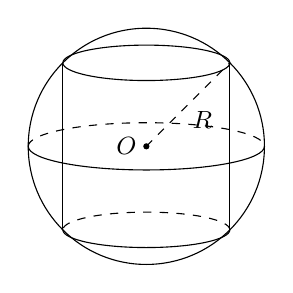
\begin{tikzpicture}[scale=0.75,font=\small]
\draw (0,0) circle (2); \draw[dashed] (-2,0) arc (180:0:2 and 0.4); \draw (-2,0) arc (180:360:2 and 0.4);
\draw (0,1.414) ellipse (1.414 and 0.3); \draw (-1.414,-1.414) arc (180:360:1.414 and 0.3); \draw[dashed] (1.414,-1.414) arc (0:180:1.414 and 0.3);
\draw (-1.414,-1.414)--(-1.414,1.414); \draw (1.414,-1.414)--(1.414,1.414); \draw[dashed] (0,0)--(1.414,1.414); \fill (0,0) circle (1.5pt);
\node[left] at (0,0) {$O$}; \node at (0.95,0.45) {$R$};
\end{tikzpicture}}
\AB{Silindrning yon sirtini toping.}{Şar radiusining silindr balandligiga nisbatini toping.}}
\QQ{45}{Yon sirti $80\pi$ ga, asosining radiusi $4$ ga teng bölgan silindr idiş suv bilan töla töldirilgan (1-rasm, $ABCD$ — silindrning öq kesimi, $O$ — pastki asos markazi). Idişning yuqori asosiga mahkamlangan ingiçka ip yordamida radiusi $3$ ga teng bölgan temir şarça suvga töliq botirildi (2-rasm, $O_1$ — şar markazi). Bunda şarça egallagan hajmdagi suv idişdan tökilib ketdi. Söngra şarça suvdan qayta olindi va idişdagi suv sathi $EF$ holatgaça pasaydi (3-rasm). $FC=x$ — suv sathining pasayiş balandligi.
\qfig{\begin{tikzpicture}[scale=0.3,font=\small]
\foreach \s/\lab in {0/1,13/2,26/3} {\begin{scope}[xshift=\s cm]
\ifnum\lab=3 \fill[qfill] (-4,0) arc (180:360:4 and 1)--(4,7.75) arc (0:-180:4 and 1)--cycle; \fill[qfill!60] (0,7.75) ellipse (4 and 1);
\else \fill[qfill] (-4,0) arc (180:360:4 and 1)--(4,10) arc (0:-180:4 and 1)--cycle; \fill[qfill!60] (0,10) ellipse (4 and 1); \fi
\draw (0,10) ellipse (4 and 1); \draw (-4,0)--(-4,10); \draw (4,0)--(4,10); \draw (-4,0) arc (180:360:4 and 1); \draw[dashed] (4,0) arc (0:180:4 and 1);
\draw[-{Stealth[length=3pt]}] (0,0)--(4,0); \fill (0,0) circle (4pt); \node[above] at (2,0) {\scriptsize$4$}; \node[below left] at (0,0) {\scriptsize$O$};
\node[left] at (-4,0) {\scriptsize$A$}; \node[right] at (4,0) {\scriptsize$B$}; \node[right] at (4,10) {\scriptsize$C$}; \node[left] at (-4,10) {\scriptsize$D$};
\node[below] at (0,-1.4) {\scriptsize\bfseries\lab-rasm};
\end{scope}}
\begin{scope}[xshift=13cm]
\fill[white,opacity=0.5] (0,3) circle (3); \draw (0,3) circle (3); \draw (-3,3) arc (180:360:3 and 0.6); \draw (0,6)--(0,10); \draw (0,3)--(3,3); \fill (0,3) circle (4pt); \node[above] at (1.5,3) {\scriptsize$3$}; \node[left] at (0,3) {\scriptsize$O_1$};
\end{scope}
\begin{scope}[xshift=26cm]
\draw[dashed] (0,7.75) ellipse (4 and 1); \node[left] at (-4,7.75) {\scriptsize$E$}; \node[right] at (4,7.75) {\scriptsize$F$}; \node[right] at (4,8.9) {\scriptsize$x$};
\end{scope}
\end{tikzpicture}}
\AB{Şar hajmining silindr hajmiga nisbatini toping.}{Şar olingandan keyin idişdagi suv sathi qançaga pasaygan?}}
\Javoblar{C B B C C C D A D B C B C D A B A A B C A D A B C A D A A B C D B C A}{\OK{36}{$1$}{$4$}\OK{37}{$\dfrac{2\pi}3$}{$5$}\OK{38}{$\dfrac13$}{$\dfrac{3\sqrt3}2$}\OK{39}{$\dfrac12$}{$-\dfrac1{16}$}\OK{40}{$\dfrac25$}{$\dfrac{27}2$}\OK{41}{$10\sqrt3$}{$\dfrac{\sqrt{21}}3$}\OK{42}{$5$}{$\dfrac{325}{24}$}\OK{43}{$3$}{$45\sqrt3$}\OK{44}{$8\pi$}{$\dfrac{\sqrt2}2$}\OK{45}{$\dfrac9{40}$}{$\dfrac94$}}
